%==============================================================================
% @author Clinton Freeman <freeman@cs.unc.edu>
% @date 2014-11-26
%==============================================================================

\FloatBarrier
\section{Case Study: Incremental Delaunay Triangulation}
\label{sec:case-delaunay}

In this section, we use the workbench to implement and visualize an incremental
Delaunay triangulation algorithm~\cite{lischinski1994incremental}. The algorithm
takes as input a point set and produces as output a triangulation that is
\emph{Delaunay}: the circumcircle of any triangle in the triangulation does not
contain any input points in its interior. Our workbench already has these types
implemented, complete with visualization code for each basic operation.
After explaining how the algorithm works, we introduce the quad-edge data
structure and use it to arrive at a correct implementation. We conclude by using
the GUI to generate an input point set and run the algorithm. 

%==============================================================================

\subsection{Algorithm Overview}

[note this is mostly from lischinski\ldots will change in future drafts]

The algorithm starts with a triangle large enough to contain all input points,
and adds points into the triangulation one by one, maintaining the invariant
that the triangulation is Delaunay. Figure 2 illustrates the point insertion
process. First, the triangle containing the new point $p$ is located (2a). New
edges are created to connect $p$ to the vertices of the containing triangle
(2b). The old edges of the triangle are inspected to verify that they still
satisfy the empty circumcircle condition. If the condition is satisfied (2c) the
edge remains unchanged. If it is violated (2d) the offending edge is flipped,
that is, replaced by the other diagonal of the surrounding quadrilateral. In
this case two more edges become candidates for inspection (edges $a$ and $b$ in
Figure 2e.) The process continues until no more candidates remain, resulting in
the triangulation shown in Figure 2f.

% In the worst case the insertion of a point can require $O(n)$ edges to be
% flipped. However, in practice the average number of edges tested per insertion
% is small (< 9). Guibas, Knuth, and Sharir have shown that if the insertion order is
% randomized, the expected time is O(1) per insertion (Guibas et al. 1990).

Locating the containing triangle can be done in an optimal $O(\log n)$ time, but
this requires maintaining complicated data structures. Alternatively, the
triangle can be located by starting from an arbitrary place in the triangulation
and moving in the direction of $p$ until the containing triangle is reached.
This requires $O(n)$ time, but if the inserted points are uniformly distributed,
the expected number of operations to locate a point is only $O(n^{1/2})$. A
simple improvement is to always resume the search from the triangle that was
found last: in this way, when the points to be located are near each other, the
containing triangles are determined quickly.

% Figure 3 shows the DT and the corresponding VD produced by this algorithm from
% 250 random points in the unit square. Note that because the quad-edge data
% structure represents both the triangulation and its dual, the topology of the
% Voronoi diagram is readily available from the DT constructed by the algorithm.
% To have a complete VD one only needs to compute the circumcenters of all the
% triangles (i.e., the locations of the Voronoi vertices.)

% A \emph{polyline} $P$ is a polygonal chain of vertices $p_1, p_2, \ldots, p_n$
% connected by line segments $\seg{p_ip_{i+1}}$ for $1 \leq i < n$. $P$ is
% \emph{simple} if the only intersection between segments is at their shared endpoints.
% Melkman's algorithm incrementally computes the convex hull of a simple polyline
% in $O(n)$ time. 
% 
% The algorithm stores the hull's vertices in a doubly-ended queue (deque) and
% maintains the invariant that they are stored in ccw order from head to tail,
% starting and ending with the most recent vertex added to the hull. The algorithm
% establishes the invariant initially by forming the deque with $p_2, p_1, p_2$ to
% represent the convex hull of the first two points. 
% 
% Now, suppose we wish to add $p_i$ to the hull. Let $v, w$ be the vertices at the
% tail of the deque and $u, v$ be the vertices at the head. Thus, $v$ is the most
% recent vertex added to the hull, and we can speak of edges $\seg{uv}$ and
% $\seg{vw}$ as being at the head and tail of the deque, respectively. 
% 
% If $p_i$ is not left of $\seg{uv}$ or inside $\seg{uv}$, then remove edge
% $\seg{uv}$ from the convex hull by popping the head of the deque; continue until
% $p_i$ is left of the edge at the head. Similarly, if $p_i$ is not left of
% $\seg{vw}$ or inside $\seg{vw}$, then remove edge $\seg{vw}$ from the convex
% hull by popping the tail of the deque; continue until $p_i$ is left of the edge
% at the tail. Finally, push $p_i$ onto both the head and tail of the deque to
% restore the invariant.
% 
% On the other hand, if $p_i$ is left or inside both $\seg{uv}$ and $\seg{vw}$,
% then we can observe that $p_i$ is not on the convex hull: because the polyline
% from $v$ to $p_i$ does not cross the polyline from $u$ to $v$ or from $v$ to
% $w$, $p_i$ can leave the hull $CH(P_{i-1})$ only by crossing $\seg{uv}$ or
% $\seg{vw}$. Hull $CH(P_{i-1})$ is identical with $CH(P_i)$, and the invariant
% already holds.

%==============================================================================

\subsection{Algorithm Implementation}

The incremental DT algorithm involves one geometric object (a subdivision), and
requires a single degree-four predicate to check whether a point is in, on, or
outside the circle defined by three points. The DDAD workbench provides the
geometric type (\texttt{Subdivision\_2r}) and the predicate
(\texttt{InCircle\_2r}). 

% The quad-edge data structure (Guibas and Stolfi 1985) was designed for
% representing general subdivisions of orientable manifolds. It is similar to the
% winged-edge data structure (Baumgart 1975), but it simultaneously represents
% both the subdivision and its dual. Each quad-edge record groups together four
% directed edges corresponding to a single undirected edge in the subdivision and
% to its dual edge (Figure 1a). Each directed edge has two pointers: a next
% pointer to the next counterclockwise edge around its origin, and a data pointer
% to geometrical and other nontopological information (such as the coordinates of
% its origin.) 
% 
% Figures 1b and 1c illustrate how three edges incident on the same
% vertex are represented using the quad-edge data structure: the vertex itself
% corresponds to the inner cycle of pointers in Figure 1c. The remaining three
% cycles correspond to the three faces meeting at the vertex.
% 
% Aside from a primitive to create an edge (MakeEdge), a single topological
% operator Splice is defined that can be used to link disjoint edges together as
% well as to break two linked edges apart. This operator is its own inverse and
% together with MakeEdge it can be used to construct any subdivision.

% Melkman's algorithm involves two geometric objects (polylines and polygons), and
% requires only a single degree-two predicate to check whether a point is to the
% left or inside of a directed line segment. The DDAD workbench provides both
% geometric types (\texttt{Polyline\_2r} and \texttt{Polygon\_2r}), and the
% predicate \texttt{RIsLeftOfOrInsidePQ}. Both geometric types are built using a
% deque as an underlying data store, so we will have the push and pop
% capabilities we need. All two dimensional geometric types are given methods to
% set the $z$ coordinate (or \emph{z-order}) of all its vertices so that users can
% draw some objects above or below others. 
% 
% The final type we must use is \texttt{IGeometryObserver}. All DDAD geometric
% types are built to be observed by other types that implement the
% \texttt{IGeometryObserver} interface. Geometric algorithm implementations that
% wish to be visualized will usually be a free function with an
% \texttt{IGeometryObserver} as the last input argument. The only thing we need to
% do with the \texttt{observer} is to have it observe the output polygon before we
% perform any operations it.
% 
% Code listing~\ref{melkman-function} shows \texttt{Melkman}, the final 
% implementation of Melkman's algorithm. The function takes as input a 
% \texttt{Polyline\_2r} and an \texttt{IGeometryObserver}, and produces as output
% a \texttt{Polygon\_2r} object. All branching tests make use of the
% \texttt{RIsLeftOrInsidePQ} predicate. Aside from a few lines setting up colors,
% z-order, and observing the output hull, the implementation is a straightforward
% transcription of the algorithm, uncluttered by visualization code. Of course,
% the visualization code must exist somewhere; we cover the high level mechanics
% in section~\ref{sec:workbench-architecture} and the specific details of the
% polyline and polygon types in section~\ref{sec:polyline-polygon}.
%  
% \lstinputlisting[float,caption=Melkman
% implementation,label=melkman-function]{code-samples/melkman.cpp}

%==============================================================================

\subsection{Generating Input Data and Executing Incremental Delaunay} 

% The workbench GUI is composed of a toolbar and two views: orthographic and
% perspective. The toolbar contains input buttons and a button for turning
% snapping on and off. The orthographic view contains an integer grid and allows
% the user to zoom and pan the camera. The perspective view renders the scene in
% 3D and allows the user to move and rotate the camera.
% 
% \begin{figure}[htb]
% 	\centering
% 	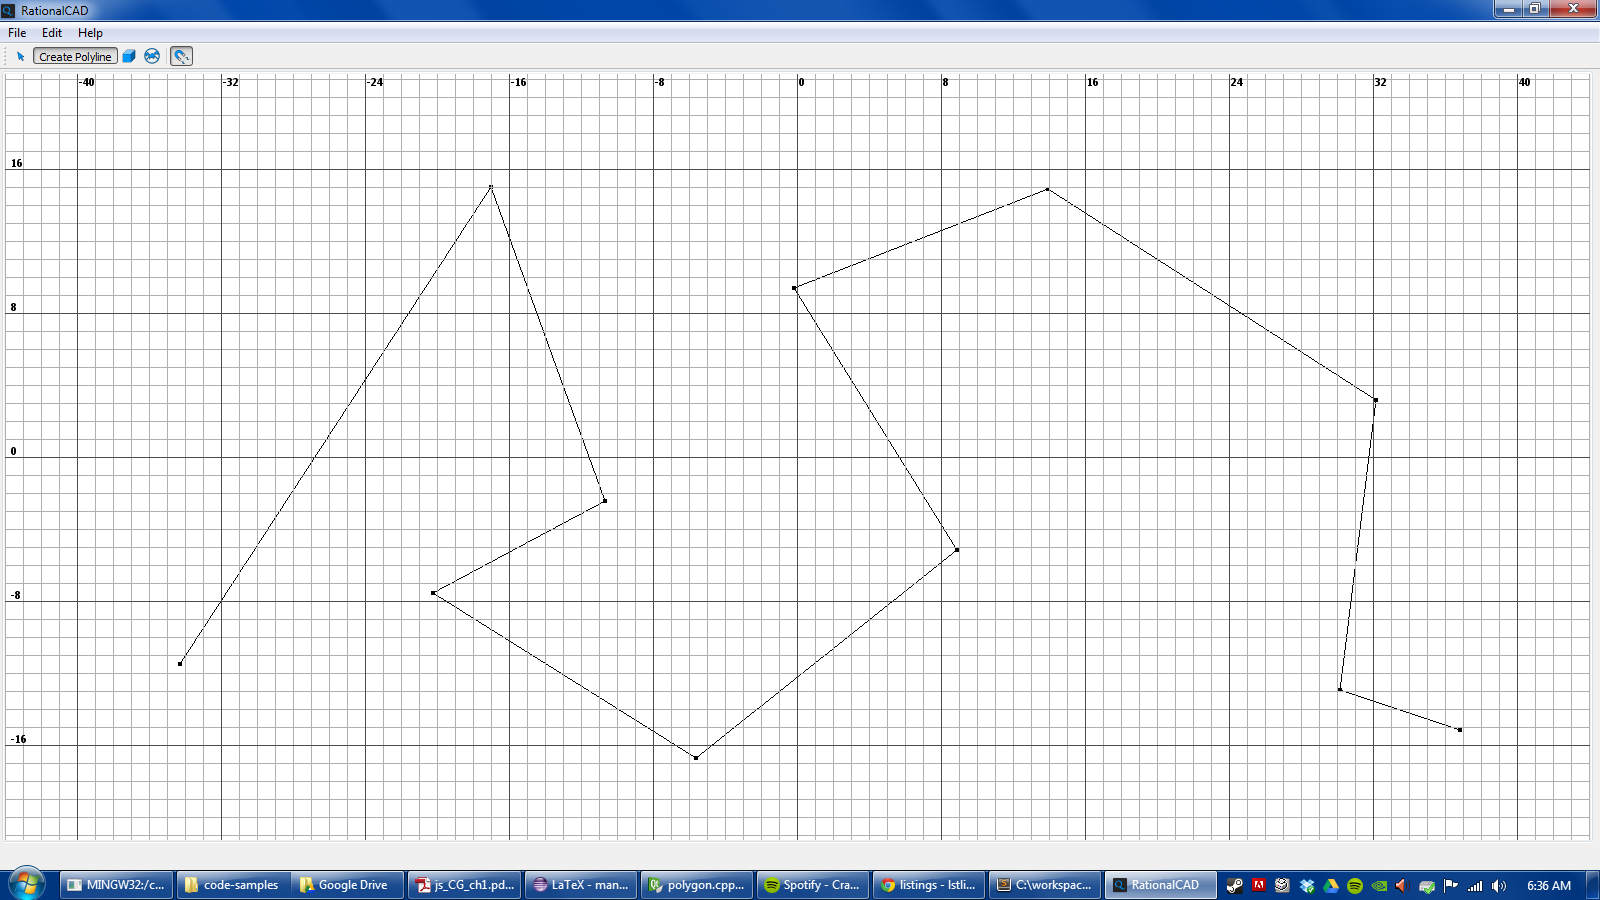
\includegraphics[width=\textwidth]{figures/melkman-input-1}
% 	\caption{Input polyline with Melkman listed in the context menu.} 
% 	\label{fig:melkman-input}
% \end{figure}
% 
% \begin{figure}[htb]
% 	\centering
% 	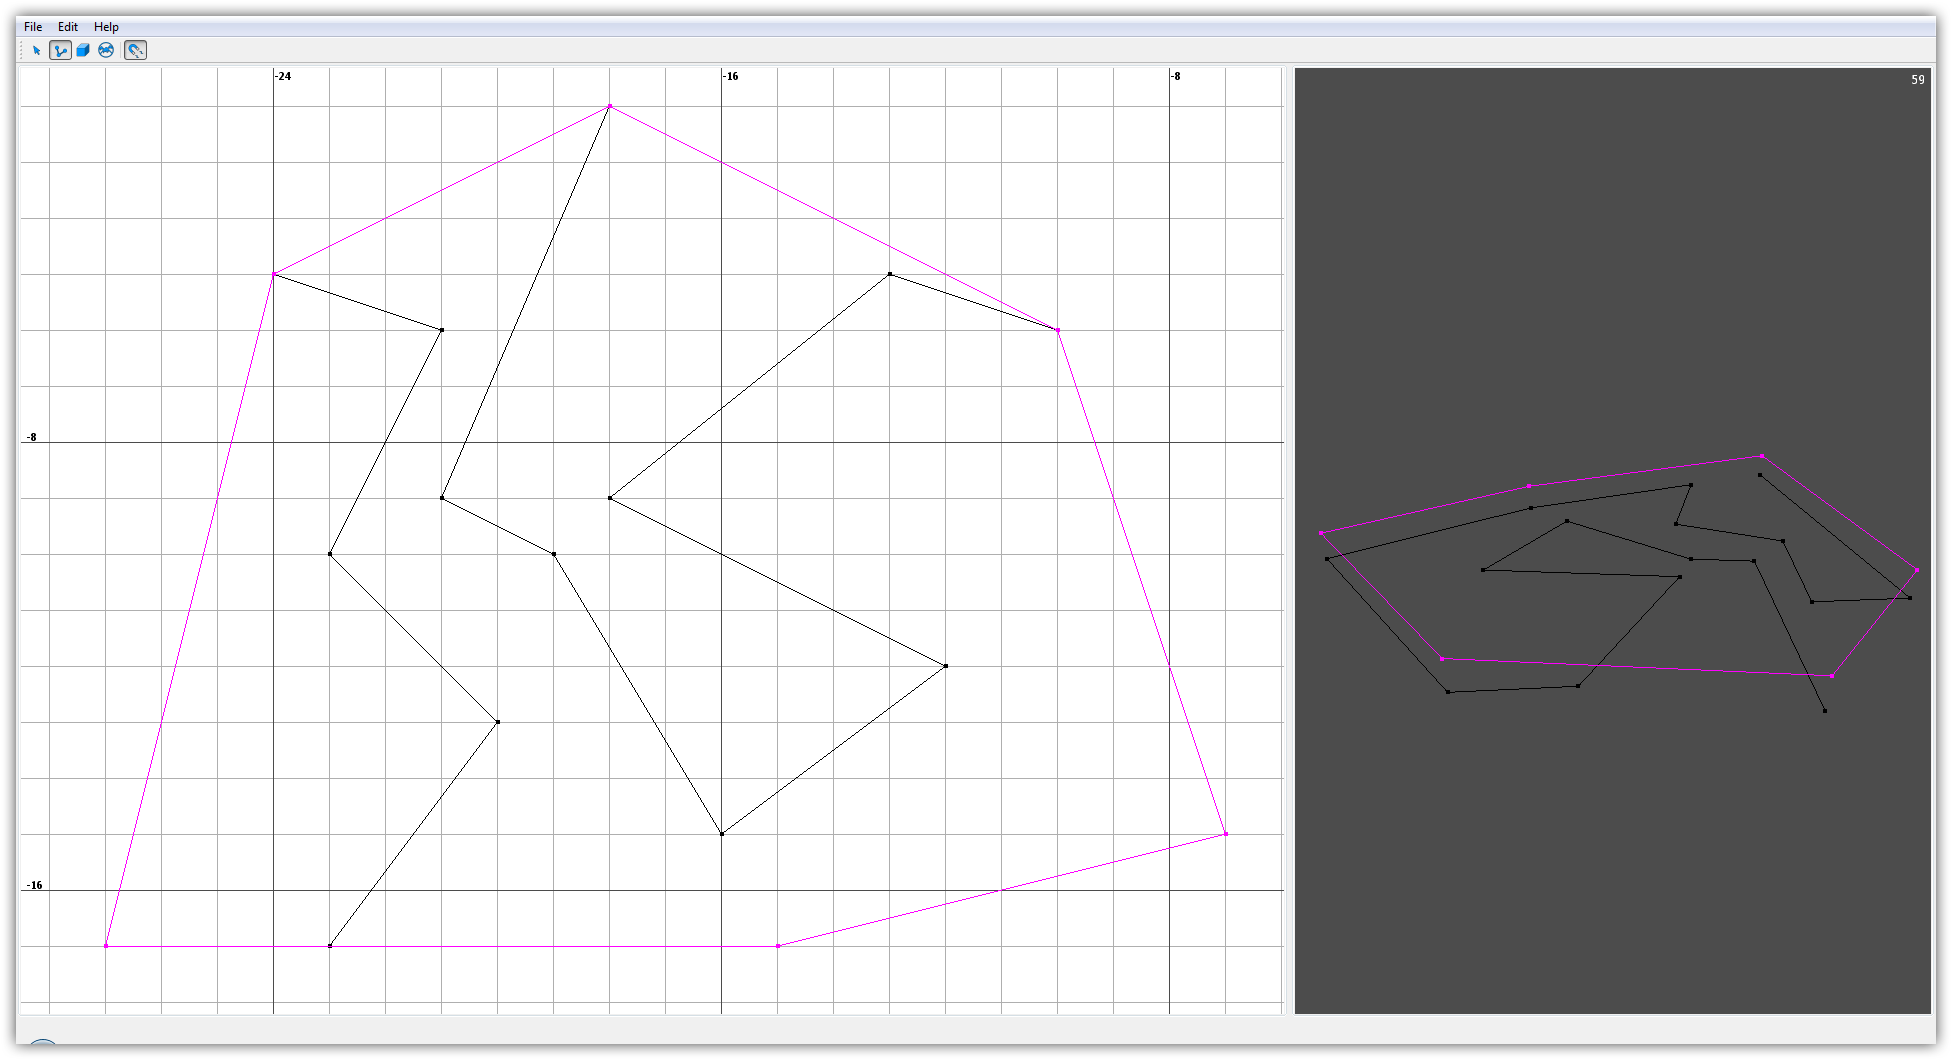
\includegraphics[width=\textwidth]{figures/melkman-output-1}
% 	\caption{Output polygon drawn on top of input polyline.} 
% 	\label{fig:melkman-output}
% \end{figure}  
% 
% The orthographic view provides a simple CAD interface, and the input buttons
% control which objects are created when the user clicks inside the view. One
% button allows the user to create polylines. The snapping toggle button
% determines whether the points created are integral. 
% 
% After clicking a few times to create a polyline, the user completes the object
% by right-clicking, and the polyline remains selected. Right-clicking again
% reveals a menu with various algorithms listed. With a few lines of code, we can 
% add Melkman to the list and specify that our new function should execute on
% the currently selected object when we click on it. 

%==============================================================================

% The DDAD workbench makes it easy for presenters and implementers to quickly
% visualize new geometric objects and algorithms. In this section, we overview
% using the workbench to implement a bare-bones visualization of Melkman's convex
% hull algorithm~\cite{melkman1987line}. First, we implement the basic data
% types used by the algorithm and augment their methods with visualization
% code. Second, we use these data types to implement Melkman's algorithm. 
% By visualizing the data types in an object-oriented way, we arrive at a
% clean implementation of the algorithm.

% The DDAD workbench can quickly visualize three-dimensional algorithms. In this
% section, we use the workbench to visualize an implementation of incremental
% delaunay triangulation. The presentation follows the same format as our previous
% case study. First, we review the basic data types used by the algorithm and
% show how to augment their methods with visualization code. Second, we use these
% data types to implement the algorithm.

%\subsection{Data Type Design and Implementation}



% This section reviews animating an incremental Delaunay triangulation algorithm.
% The algorithm is covered extensively in \cite{de2000computational}.  

%\subsection{Algorithm Overview}

% The algorithm uses the quadedge data structure~\cite{guibas1985primitives}.
% 
% \begin{mdframed}[linecolor=white, backgroundcolor=algback, frametitle={Algorithm
% Delaunay}] \begin{algorithmic}[1]
%     \Require A set $P$ of $n+1$ points in the plane.
%     \Ensure A Delaunay triangulation of $P$.
%     \vspace{0.75em}
%     \Procedure{Delaunay}{$P$}
%     \State Let $p_0$ be the lexicographically highest point of $P$.
%     \State Let $p_{-1}, p_{-2}$ be two points far away such that $P$ is
%     contained in the triangle $p_0p_{-1}p_{-2}$.
%     \State Initialize $\mathcal{T}$ as the triangulation consisting of the
%     single triangle $p_0p_{-1}p_{-2}$.
%     \State Compute a random permutation $p_1, p_2, \ldots, p_n$ of $P /
%     \{p_0\}$.
%     \For{$r = 1 \ldots n$}
%    \State derp
%     \EndFor \EndProcedure
% \end{algorithmic}
% \end{mdframed} 

% \subsection{Code Listing}
% 
% \lstinputlisting{code-samples/delaunay.cpp}
% 
% \subsection{Generating Input Data}
% 
% The user is given a button in the GUI and may browse to read in point sets
% stored in text files.
